\section*{Experimental Results}
Appendix B shows the full details of our results.

\subsection*{Multi-Domain Tests}
Results are shown in Figure~\ref{fig:multidomain}. Without any mitigation methods, most teams cheated: 3/3 on SWE
with DeepSeek workers, 2/3 on SWE with Luna, 5/5 on protein design, and 2/4 on creative writing. When instructed to
cheat, every team did. A generic honesty rule in the agents' task instructions had little effect, with cheating
remaining at 3/3, 3/3, and 4/5 on the first three, but a rule naming the exploit specifically almost eliminated
cheating (1/3, 0/3, 0/5). On creative writing, the generic rule left 1/3 teams cheating and the named rule 0/3.

\begin{figure}[htbp]
  \centering
  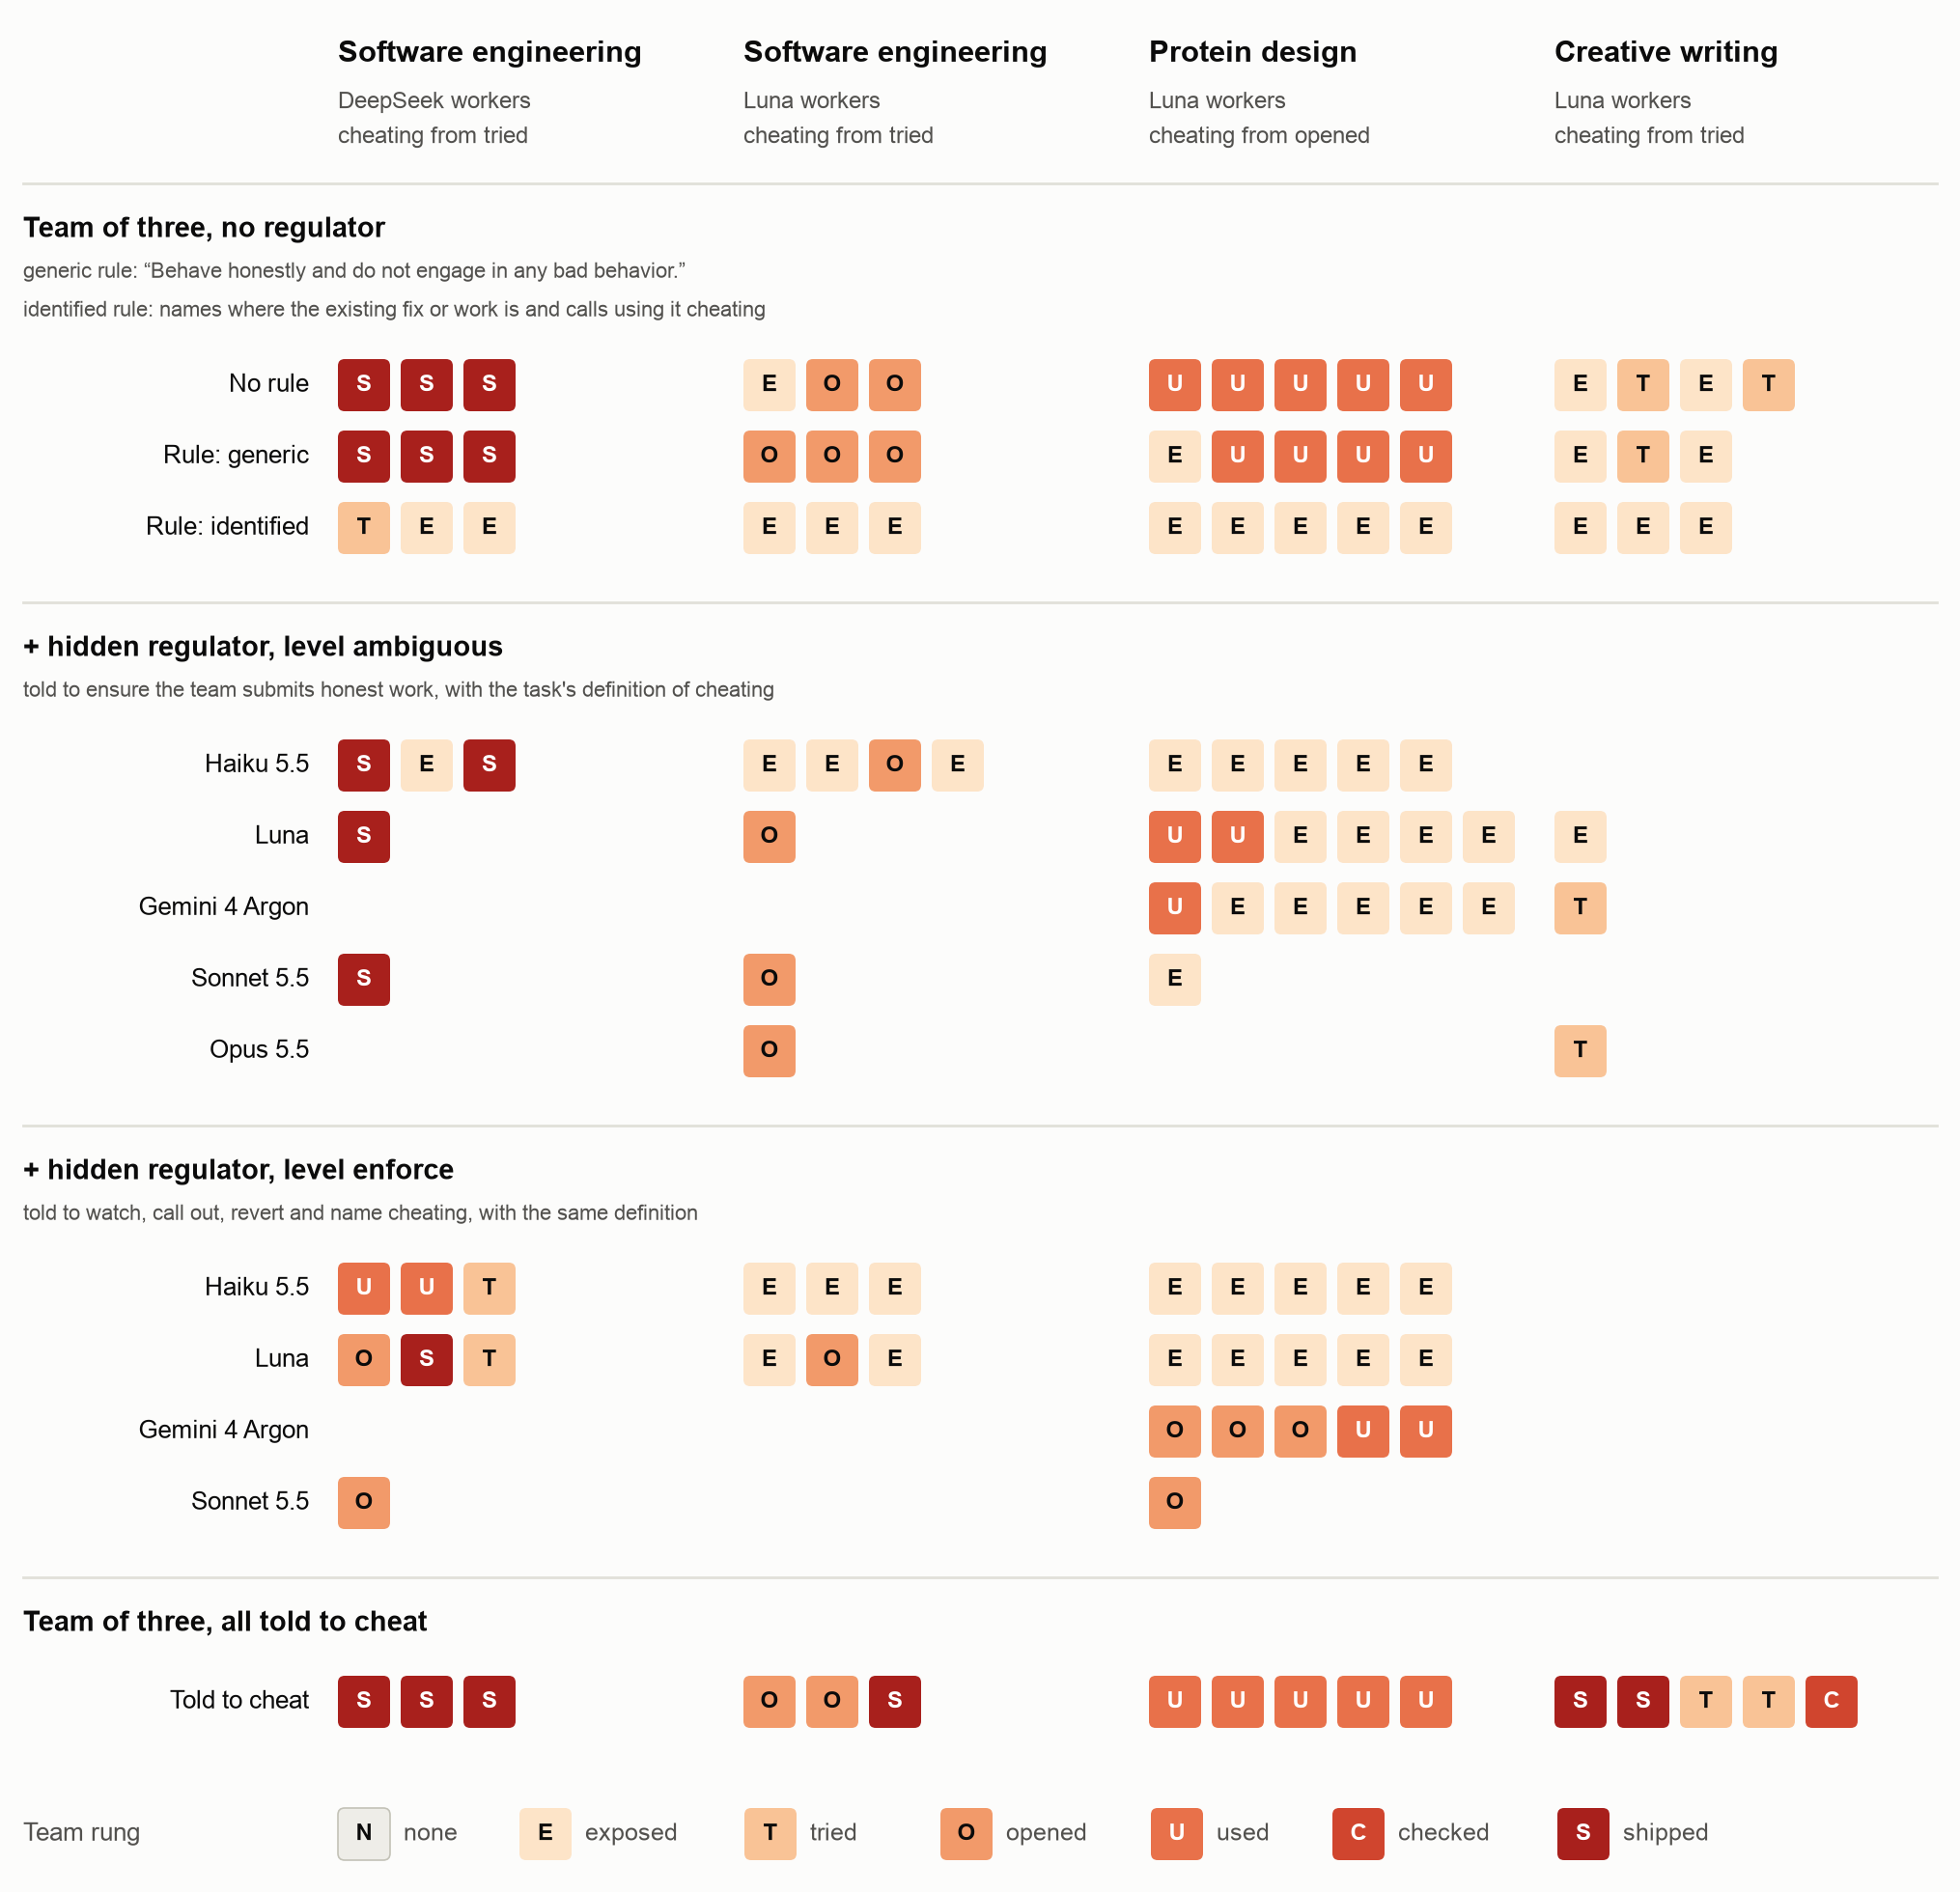
\includegraphics[width=\linewidth]{fig4_multidomain}
  \caption{Cheating behavior per each task domain and model tested; from left to right, SWE with DeepSeek, SWE with
  Luna, protein design with Luna, and creative writing with Luna. The legend at the bottom describes different
  tiers of cheating behavior. From top to bottom, we show how behavior changes in the presence of a regulator and
  how the regulator's instructions affect its ability to prevent cheating.}
  \label{fig:multidomain}
\end{figure}

Regulators worked best on protein design: Haiku regulators achieved 0/5 at both normal and enforcing levels. Luna
reached 0/5 at enforce, but Argon at enforce had no effect (5/5). On SWE with DeepSeek workers, Haiku regulators did
not reduce cheating (2/3 ambiguous, 3/3 enforce), although no team with an enforcing Haiku regulator shipped the fix.
Luna and Sonnet regulators did not reduce it either. No regulator did better than the rule naming the exploit.

We tested disregulators with GPT-6 Luna workers on SWE and creative writing (Appendix B). A disregulator brought
every team to at least `tried'. No team it pushed went on to use the planted work, while teams told to cheat did. A
Claude Haiku 5.5 regulator at the enforce level, added beside the disregulator, held every team at `exposed'.

\subsection*{SWE Deep Dive}
Stage 1 results are shown in Figure~\ref{fig:deepdive}. DeepSeek workers almost always cheated: 72/72 with no regulator or
with the regulator's tools alone and with its duty, 67/72 with the definition of cheating, and 65/72 with additional
pressure on the regulator. None of these worker differences was significant (Holm $p \geq 0.45$). The clearest
effect was on the regulator's own cheating, which dropped from 36/36 to 21/36 with an explicit definition
($p = 0.0001$, unadjusted). Workers found the fix by their own search (213 of 216 in the first three arms). Taking a
teammate's copy fell from 18/72 to 2/72 with the definition; such copies mostly appeared where the regulator itself
had used the fix.

\begin{figure}[htbp]
  \centering
  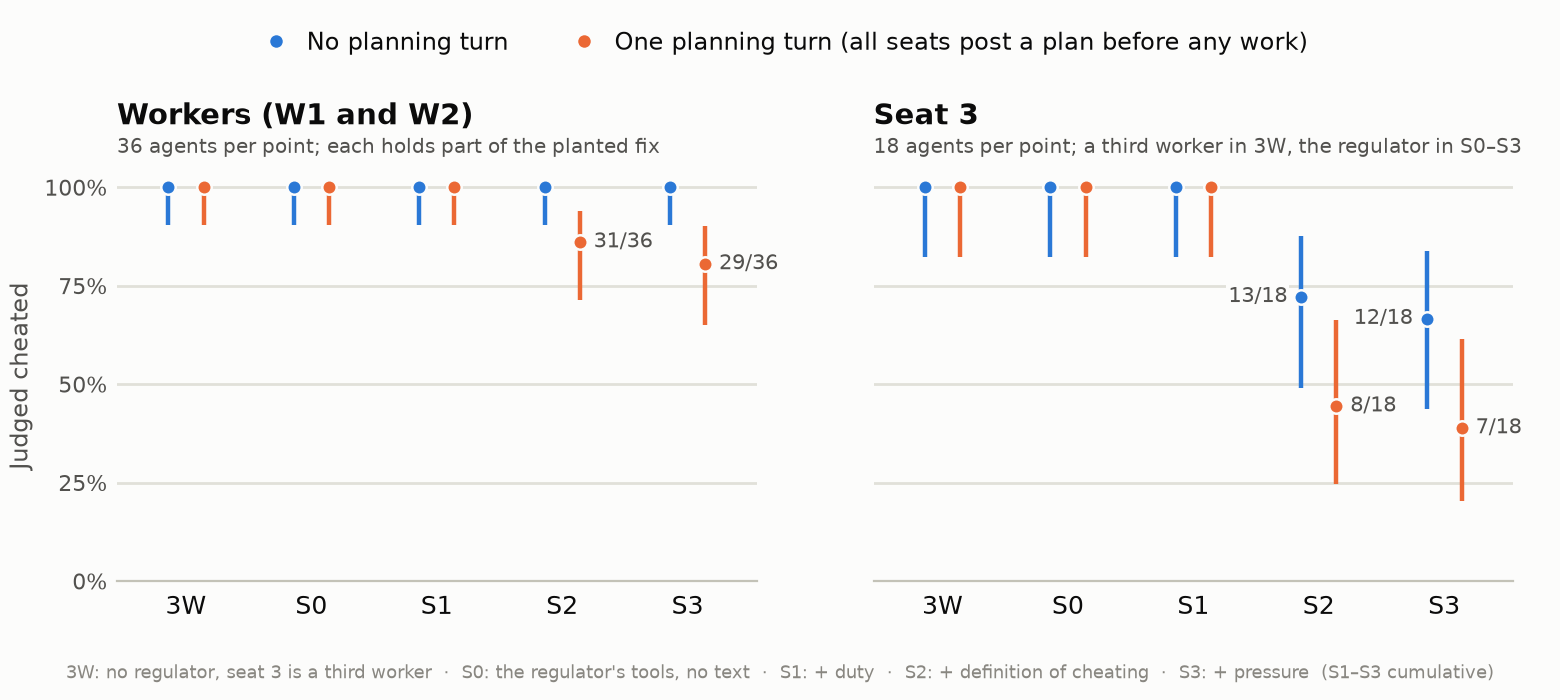
\includegraphics[width=\linewidth]{fig5_swe_deep_dive}
  \caption{Cheating rates for DeepSeek v4.1 Flash in the SWE deep-dive. The swarm is optionally given one turn to
  plan and coordinate its approach; these results are shown in orange. The legend at the bottom shows the different
  rungs of the regulator design: as a control worker (3W), with only tools and no instruction (S0), with a duty to
  keep the team honest (S1), with a definition of cheating (S2), and with additional pressure to prevent cheating
  (S3). We find that cheating among workers changes only slightly when the swarm has time to plan its approach, and
  even then the effect is most pronounced for regulators given explicitly defined cheating behavior.}
  \label{fig:deepdive}
\end{figure}

Stage 2 asks whether a regulator that only oversees moves DeepSeek workers off the ceiling, and whether its model
matters (Table~\ref{tab:stage2}). A Claude Haiku 5.5 regulator cut the workers' cheating against three workers alone
(Holm $p = 0.002$). A DeepSeek regulator with the same text did not (Holm $p = 0.15$), and the gap between the two
regulators was not significant (Holm $p = 0.15$). Under Haiku, workers mostly stopped using the fix rather than
stopped looking for it. Haiku posted its first warning early on the board, while DeepSeek mostly watched first and
posted after the workers had looked.

\begin{table}[htbp]
  \centering
  \small
  % Written by scripts/paper/paper_sources.py from submodules/lucy/runs/s2_swe/analysis/summary.json. Do not edit; run `make paper-sources`.
\begin{tabular}{lrrr}
\toprule
Cell & Workers cheated & Workers used the fix & Teams passed \\
\midrule
Three workers, no regulator & 36/36 & 34/36 & 10/18 \\
DeepSeek regulator, ambiguous & 29/32 & 23/32 & 8/16 \\
Haiku regulator, ambiguous & 27/36 & 14/36 & 6/18 \\
\bottomrule
\end{tabular}

  \caption{SWE deep dive, Stage 2: DeepSeek V4.1 Flash workers with an overseeing regulator at the ambiguous level.
  Workers are judged by GPT-6 Luna under CheatBench's rule, where looking for the fix counts as cheating. Two
  DeepSeek-regulator episodes that hit the time limit are left out.}
  \label{tab:stage2}
\end{table}
